
\documentclass[10pt]{article}

\usepackage[utf8]{inputenc}
\usepackage{xcolor}
\usepackage{float}
\usepackage{graphicx}
\usepackage{geometry}
\usepackage{float}
\usepackage[toc,page]{appendix}
\graphicspath{ {./images/} }
\parindent=0pt
\usepackage{hyperref}
\hypersetup{
  colorlinks = true,
  linkcolor = blue,
  citecolor=blue,
  linkbordercolor = {white},
}
\usepackage{fullpage}
\usepackage{fancyvrb}

\frenchspacing

\usepackage{microtype}

\usepackage[english,dutch]{babel}

\usepackage{listings}
% Er zijn talloze parameters ...
\lstdefinestyle{myStyle}{
  belowcaptionskip=1\baselineskip,
  breaklines=true,
  frame=none,
  numbers=left, numberstyle=\tiny, numberfirstline=false, breaklines=true,
  stepnumber=1, tabsize=8,
  basicstyle=\footnotesize\ttfamily,
  keywordstyle=\bfseries\color{blue!40!black},
  commentstyle=\itshape\color{green!40!black},
  identifierstyle=\color{black},
}

\usepackage{caption}
\usepackage{subcaption}

\title{Opdracht 3}
\author{Jenny Vermeltfoort}

\begin{document}

\selectlanguage{dutch}
\def\tablename{Tabel}

\maketitle

\section{Gebruik}

De speler van het spel kan het volgende:
\begin{enumerate}
  \item de breedte en lengte van het bord configureren.
  \item het aantal bommben configureren.
  \item het programma stoppen,
  \item een vlag plaatsen of verwijderen met 'f' als input.
  \item een vakje openen met spatie als input.
  \item een cursor over het bord verplaatsen met 'h,j,k,l' als inputs.
  \item na een zet, de staat van het vorige bord terughalen, ook wanneer de speler dood is gegaan.
  \item een automatische robot configureren, die random zetten speelt. De resultaten worden geplaatst in de output
        file. De speler kan het aantal iteraties configureren.
\end{enumerate}

\section{Resultaten}
De Minesweeper robot is met de volgende configuraties gedraaid:
\begin{itemize}
  \item De verschillende bord maten: 9x9, 15x15 en 20x20.
  \item Alle maten met verschillende hoeveelheden bommen: 50 of 20 bommen. Dit is bij 9x9,
        60\% en 25\%; bij 15x15, 22\% en 9\%; bij 20x20, 12.5\% en 5\%.
  \item 100.000 potjes per configuratie.
\end{itemize}

Een aantal resultaten zijn zichtbaar in fig. \ref{fig:plots}. Het is opvallend dat bord maten vijftien bij vijftien en
twintig bij twintig geen
gewonnen potjes heeft bij vijftig bommen; en met een configuratie van twintig bommen winnen ze beiden binnen 6 zetten,
zie
fig. \ref{fig:plot_15_15_won} en fig. \ref{fig:plot_20_20_won}. Verder duurt een potje maximaal twintig tot
vijfentwintig zetten, te
zien in fig. \ref{fig:plot_9_9_total} en fig. \ref{fig:plot_20_20_total}. De robot verliest bij het negen bij negen
bord ongeveer in 25\%  meer
zetten dan dat het wint. Dit is 22\% bij 20 bommen en 28\% bij 50 bommen, zie fig. \ref{fig:plot_9_9_won} en fig.
\ref{fig:plot_9_9_lost}.

\hfill
\begin{figure}[H]
  \centering
  \begin{subfigure}{.49\textwidth}
    \centering
    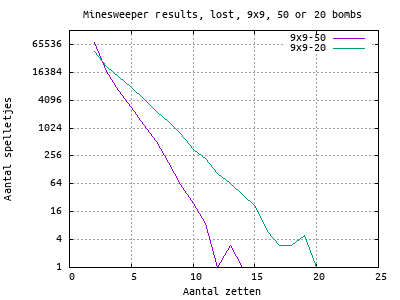
\includegraphics[width=1\linewidth]{plot_9_9_lost}
    \caption{Resultaat verloren, 9x9. }
    \label{fig:plot_9_9_lost}
  \end{subfigure}
  \begin{subfigure}{.49\textwidth}
    \centering
    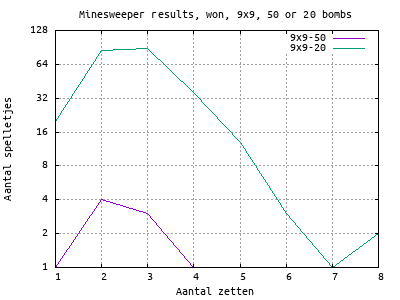
\includegraphics[width=1\linewidth]{plot_9_9_won}
    \caption{Resultaat gewonnen, 9x9. }
    \label{fig:plot_9_9_won}
  \end{subfigure}
  \begin{subfigure}{.49\textwidth}
    \centering
    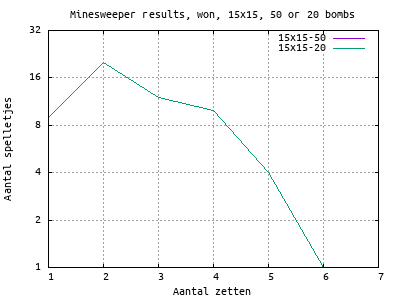
\includegraphics[width=1\linewidth]{plot_15_15_won}
    \caption{Resultaat gewonnen, 15x15. }
    \label{fig:plot_15_15_won}
  \end{subfigure}
  \begin{subfigure}{.49\textwidth}
    \centering
    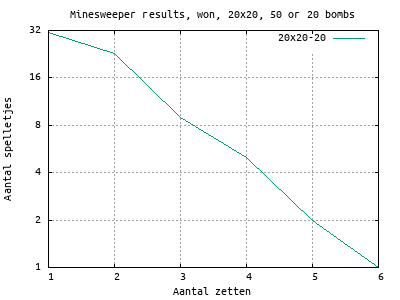
\includegraphics[width=1\linewidth]{plot_20_20_won}
    \caption{Resultaat gewonnen, 20x20. }
    \label{fig:plot_20_20_won}
  \end{subfigure}
  \begin{subfigure}{.49\textwidth}
    \centering
    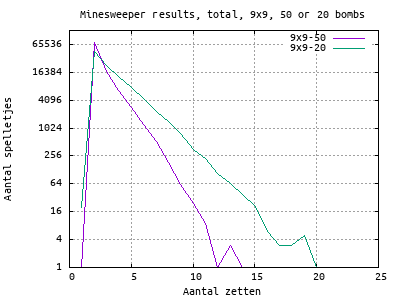
\includegraphics[width=1\linewidth]{plot_9_9_total}
    \caption{Resultaat totaal, 9x9. }
    \label{fig:plot_9_9_total}
  \end{subfigure}
  \begin{subfigure}{.49\textwidth}
    \centering
    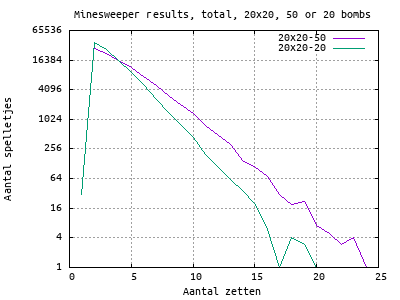
\includegraphics[width=1\linewidth]{plot_20_20_total}
    \caption{Resultaat totaal, 20x20. }
    \label{fig:plot_20_20_total}
  \end{subfigure}
  \caption{Resultaten}
  \label{fig:plots}
\end{figure}

\section{Tijd}
Zie tabel \ref{tab:time} voor de tijd verantwoording.

\begin{table}[H]
  \begin{center}
    \begin{tabular}{ l c }
      Week & Uur \\ \hline
      42   & 8   \\
      43   & 4   \\
      45   & 8   \\
    \end{tabular}

    \caption{Tijd verantwoording}
    \label{tab:time}
  \end{center}
\end{table}

\bibliographystyle{ieeetr}
\bibliography{bibtex.bib}

\newgeometry{left=2cm,bottom=2cm,top=2cm, right=2cm}
\newpage
\begin{appendices}
  \section{Code}\label{sec:code}
  \lstinputlisting[caption=main.cpp,
    language=C++,
    style=myStyle]{../src/main.cpp}

  \lstinputlisting[caption=board.hpp,
    language=C++,
    style=myStyle]{../src/board.hpp}

  \lstinputlisting[caption=board.cpp,
    language=C++,
    style=myStyle]{../src/board.cpp}

  \lstinputlisting[caption=handler.hpp,
    language=C++,
    style=myStyle]{../src/handler.hpp}

  \lstinputlisting[caption=handler.cpp,
    language=C++,
    style=myStyle]{../src/handler.cpp}

  \lstinputlisting[caption=stack.hpp,
    language=C++,
    style=myStyle]{../src/stack.hpp}

  \lstinputlisting[caption=stack.cpp,
    language=C++,
    style=myStyle]{../src/stack.cpp}

  \lstinputlisting[caption=print.hpp,
    language=C++,
    style=myStyle]{../src/print.hpp}

  \lstinputlisting[caption=print.cpp,
    language=C++,
    style=myStyle]{../src/print.cpp}

\end{appendices}

\end{document}